\chapter{Stand der Technik}
\label{cha:stand_der_technik}

\section{RT Technik}

\subsection{Geometrische Unschärfe }
\label{sec:ndt}

Geometrische Unschärfe bezieht sich auf den Verlust der Definition, der das Ergebnis geometrischer Faktoren der radiographischen Ausrüstung und des Aufbaus ist.Es tritt auf, weil die Strahlung nicht von einem einzelnen Punkt, sondern über eine Fläche stammt.
Betrachten Sie die Bilder unten, die zwei Quellen unterschiedlicher Größe zeigen, die Strahlengänge von jeder Kante der Quelle zu jeder Kante des Merkmals der Probe, die Stellen, an denen diese Strahlung den Film belichtet, und das Dichteprofil über den Film. Im ersten Bild stammt die Strahlung von einer sehr kleinen Quelle. Da die gesamte Strahlung im wesentlichen aus dem gleichen Punkt stammt, wird im Bild sehr wenig geometrische Unschärfe erzeugt. In dem zweiten Bild ist die Quellengröße größer und die verschiedenen Wege, die die Strahlungsstrahlen von ihrem Ursprungspunkt in der Quelle nehmen können, bewirken, dass die Kanten der Einkerbung weniger definiert sind.\\
\subsubsection{GeometricUnsharpness}
\begin{figure}[htb]
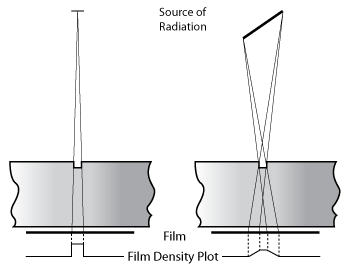
\includegraphics[scale=0.5]{img/GeometricUnsharpness.png}\\
\label{sec:GeometricUnsharpness}
  \caption{GeometricUnsharpness}
  \label{sec:geometricUnsharpness1}
  \end{figure}

Die drei Faktoren, die die Unschärfe steuern, sind die Quellengröße, die Entfernung von Quelle zu Objekt und die Distanz zwischen Objekt und Detektor. Die Quellengröße wird durch Bezugnahme auf Herstellerspezifikationen für eine gegebene Röntgen- oder Gammastrahlenquelle erhalten. Industrieröntgenröhren haben häufig Brennfleckgrößen von 1,5 mm im Quadrat, Mikrofokussysteme haben jedoch Fleckgrößen im Bereich von 30 Mikron. Wenn die Quellengröße abnimmt, nimmt auch die geometrische Unschärfe ab. Für eine Quelle mit gegebener Größe kann die Unschärfe ebenfalls durch Erhöhen der Entfernung von der Quelle zum Objekt verringert werden, dies führt jedoch zu einer Verringerung der Strahlungsintensität.
Der Abstand zwischen Objekt und Detektor wird normalerweise so klein wie möglich gehalten, um die Unschärfe zu minimieren. Es gibt jedoch Situationen, z. B. bei Verwendung einer geometrischen Vergrößerung, wenn das Objekt vom Detektor getrennt wird, was die Definition verringert. Das unten stehende Applet ermöglicht die Visualisierung der geometrischen Unschärfe, wenn Quellgröße, Entfernung von Quelle zu Objekt und Abstand zwischen Quelle und Detektor variiert werden. Der Bereich mit unterschiedlicher Dichte am Rand eines Features, der sich aufgrund geometrischer Faktoren ergibt, wird als Penumbra bezeichnet.

Codes und Standards, die in der industriellen Radiographie verwendet werden, erfordern, dass geometrische Unschärfe begrenzt wird. Im Allgemeinen beträgt die zulässige Menge 1/100 der Materialdicke bis zu einem Maximum von 0,040 Zoll. Diese Werte beziehen sich auf den Grad des Halbschattens in einem Röntgenbild.
Da die Penumbra nicht annähernd so gut definiert ist, wie in der Abbildung(\ref{sec:geometricUnsharpness})gezeigt, ist es schwierig, sie in einem Röntgenbild zu messen. Daher wird es typischerweise berechnet.
Die Quellengröße muss vom Gerätehersteller bezogen oder gemessen werden. Dann kann die Unschärfe anhand von Messungen des Setups berechnet werden.
Für den Fall, wie rechts gezeigt, wo eine Probe mit einer signifikanten Dicke in der Nähe des Detektors platziert wird, wird die folgende Formel verwendet, um die maximale Menge an Unschärfe aufgrund der Probendicke zu berechnen:\\

  Ug = f * b/a

f = Quelle Brennpunktsgröße (source focal-spot size) \\
a = Abstand von der Quelle zur vorderen Oberfläche des Objekts\\
b = Die Dicke des Objekts\\
\begin{figure}[htb]
  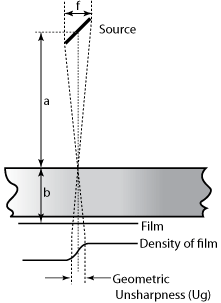
\includegraphics[scale=0.9]{img/GeometricUnsharpness2.png}\\
  \caption{GeometricUnsharpness2}
  \label{sec:geometricUnsharpness}
  \end{figure}
Für den Fall, dass der Detektor nicht neben der Probe platziert wird, etwa wenn eine geometrische Vergrößerung verwendet wird, wird die Berechnung zu:\\

Ug = f* b/a\\
f = Quelle Brennpunktsgröße (source focal-spot size) \\
a = Abstand von der Röntgenquelle(x-ray) zur vorderen Oberfläche des Materials / Objekts\\
b = Die Dicke des Objekts\\
\begin{figure}[htb]
  \centering 
 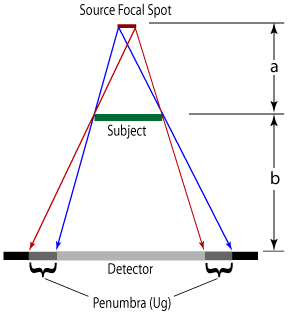
\includegraphics[scale=0.9]{img/Penumbra.png}
 \caption{Penumbra}
  \label{fig:Penumbra}
\end{figure}

\label{sec:RT Technik}
\section{Sekundäre Strahlung und Unterschnittkontrolle}
\label{sec:Strahlung und Unterschnittkontrolle}
Quelle: \url{https://www.nde-ed.org/index_flash.htm}
\subsection{Sekundäre Strahlung}
Sekundär- oder Streustrahlung muss oft bei der Erstellung eines Röntgenbildes berücksichtigt werden. Die gestreuten Photonen erzeugen einen Verlust von Kontrast und Definition. Häufig wird Sekundärstrahlung als Strahlung angesehen, die auf den Film trifft, der von einem Objekt in der unmittelbaren Umgebung, wie einer Wand, oder von dem Tisch oder Boden, auf dem das Teil ruht, reflektiert wird. Seitliche Streuung entsteht von Wänden oder Objekten auf der Quellseite des Films. Die Steuerung der Seitenstreuung kann erreicht werden, indem Objekte in dem Raum weg von dem Film bewegt werden, die Röntgenröhre in die Mitte des Gewölbes bewegt wird oder ein Kollimator an der Austrittsöffnung platziert wird, wodurch die divergierende Strahlung um den Zentralstrahl reduziert wird.
\begin{figure}[htb]
 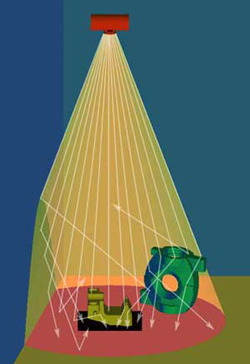
\includegraphics[scale=0.7]{img/XRSIM-Scatter2aS.jpg}
 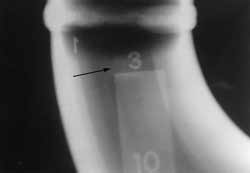
\includegraphics[scale=0.9]{img/BackScatter(small).jpg}
 \caption{BackScatter}
 Quelle: \url{https://www.nde-ed.org/index_flash.htm}
  \label{fig:BackScatter}
\end{figure}
Es wird oft als Rückstreuung bezeichnet, wenn es von Objekten hinter dem Film kommt. Industriestandards und Standards verlangen oft, dass ein Buchstabe B auf der Rückseite der Kassette platziert wird, um die Kontrolle der Rückstreuung zu überprüfen.

Wenn der Buchstabe B als ein Geister -Bild auf dem Film erscheint, erreicht eine signifikante Menge an Rückstreustrahlung den Film. Das Bild des B ist oft sehr unscharf,
(BILD \ref{fig:BackScatter}). Der Pfeil zeigt auf das Gebiet der Rückstreustrahlung von der Leitung B, die sich auf der Rückseite des Films befindet. Die Steuerung der Rückstreustrahlung wird erreicht, indem der Film in der Kassette mit einer mindestens 0,010 Zoll dicken Bleifolie hinterlegt wird. Es ist eine übliche Praxis in der Industrie, einen 0,005-Zoll-Führungsschirm vor und einen 0,010-Zoll-Schirm hinter dem Film anzuordnen.
\subsection{Unterschnitt}
Eine weitere Bedingung, die oft bei der Erstellung eines Röntgenbildes kontrolliert werden muss, ist Undercut. Teile mit Löchern, hohlen Bereichen oder abrupten Dickenänderungen werden wahrscheinlich durch Unterschnitte beeinträchtigt, wenn die Bedienelemente nicht eingesetzt werden. Hinterschnitt erscheint als Verdunkelung des Röntgenbildes im Bereich des Dickenübergangs. Dies führt zu einem Verlust der Auflösung oder Unschärfe im Übergangsbereich. Unterschneidung tritt aufgrund von Streuung innerhalb des Films auf.\\

An den Rändern eines Teils oder der Bereiche, wo der Teil von dick zu dünn übergeht, ist die Intensität der Strahlung, die den Film erreicht, viel größer als in den dickeren Bereichen des Teils. Die hohe Strahlungsintensität, die den Film erreicht, führt zu einer hohen Streuung innerhalb des Films. Es sollte auch beachtet werden, dass, je schneller die Filmgeschwindigkeit ist, desto mehr Unterschneidung wahrscheinlich auftritt. Streuung innerhalb der Wände des Teils trägt ebenfalls zur Unterschneidung bei, aber die Forschung hat gezeigt, dass die Streuung innerhalb des Films die Hauptursache ist. Masken dienen zur Kontrolle der Unterschneidung. Als Masken werden häufig Bleibleche verwendet, die zum Füllen von Löchern oder zum Umschließen des Teils geschnitten werden, und metallische Schrot- und Flüssigkeitsabsorber.

\begin{figure}[htb]
  \centering 
 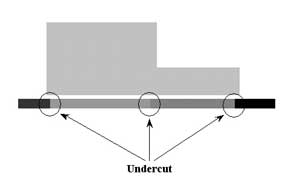
\includegraphics[scale=0.9]{img/Undercut.jpg}
 \caption{Undercut}
  \label{fig:Undercut}
  Quelle: \url{https://www.nde-ed.org/index_flash.htm}
\end{figure}
\begin{figure}[h]
 %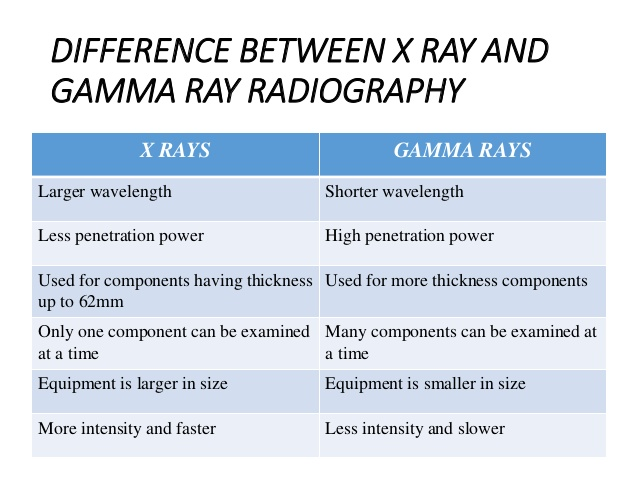
\includegraphics[scale=0.5]{img/gammaAndx-ray.jpg}
   \centering
 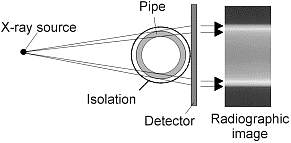
\includegraphics[scale=0.5]{img/x-ray.png}
 \caption{X-Ray}
  \label{fig:gammaAndx-ray}
  \centering
  Quelle: \url{https://www.nde-ed.org/index_flash.htm}
\end{figure}

\section{Filter in der Radiographie}
\subsection{X-Ray}

Bei Röntgenenergien bestehen Filter aus Material, das in dem Nutzstrahl angeordnet ist, um vorzugsweise Strahlung basierend auf dem Energieniveau zu absorbieren oder die räumliche Verteilung des Strahls zu modifizieren. Die Filtration wird benötigt, um die Röntgenstrahlen mit niedrigerer Energie zu absorbieren, die von der Röhre emittiert werden, bevor sie das Ziel erreichen. Die Verwendung von Filtern erzeugt ein saubereres Bild durch Absorbieren der Röntgenstrahlenphotonen mit niedrigerer Energie, die dazu neigen, mehr zu streuen.

Die Gesamtfiltration des Strahls umfasst die inhärente Filtration (bestehend aus einem Teil der Röntgenröhre und des Röhrengehäuses) und die hinzugefügte Filterung (dünne Bleche eines Metalls, das in den Röntgenstrahl eingeführt wird). Filter werden typischerweise in der Nähe des Röntgenstrahlkanals im direkten Weg des Röntgenstrahls angeordnet. Auch eine dünne Kupferfolie zwischen dem Teil und der Filmkassette hat sich als eine effektive Filtrationsmethode erwiesen.

Für die industrielle Radiographie werden die Filter, die dem Röntgenstrahl hinzugefügt werden, meistens aus Materialien mit hoher Kernladungszahl wie Blei, Kupfer oder Messing hergestellt. Filter für die medizinische Radiographie bestehen in der Regel aus Aluminium (Al). Die Menge sowohl der inhärenten als auch der zugesetzten Filtration wird in mm Al oder mm Al-Äquivalent angegeben. Die Filtrationsmenge des Röntgenstrahls wird spezifiziert durch und basiert auf dem Spannungspotential (keV), das verwendet wird, um den Strahl zu erzeugen. Die Dicke der Filtermaterialien hängt von Ordnungszahlen, Kilovolt-Einstellungen und dem gewünschten Filtrationsfaktor ab.

\subsection{Gamma}
Gammaradiographie erzeugt relativ hohe Energieniveaus bei im wesentlichen monochromatischer Strahlung, daher ist die Filtration keine nützliche Technik und wird selten verwendet.\\



\subsection{RT-Ressourcen}
\label{sec:resourcen}
\begin{enumerate}
\item Personal: mindestens 2
\begin{itemize}
\item Health Physics Safety(HPS)
\item Radiographer
\item Assistance
\end{itemize}
\item Haupt-Materialien 
\begin{itemize}
\item Materialien
\begin{itemize}
\item Radioaktive Isotope z.B. Iridium-192
\item Gamma Radiation Projection Devices z.B.
\href{https://www.ndt.com.au/product/qsa-sentinel-iridium-ir-192-sources-for-gamma-radiography/}{\textcolor{blue}{SENTINEL}}
\item Film z.B.
\href{https://www.gemeasurement.com/sites/gemc.dev/files/geit-40007-structurix_en_04-17.pdf}{\textcolor{blue}{AGFA}} 
\end{itemize}
\item Prozess-Materialien
\begin{itemize}
\item Chemikalien für Filmentwickler und Filmfixierer z.B. \href{https://www.gemeasurement.com/sites/gemc.dev/files/geit-40007-structurix_en_04-17.pdf}{\textcolor{blue}{AGFA}}
\item Dunkelkammer für Entwicklung z.B.
\href{https://www.gemeasurement.com/sites/gemc.dev/files/structurix_processing_equipment_brochure_english.pdf}{\textcolor{blue}{Digitale Dunkelkammer}}
\end{itemize}
\item Sicherheit-Materialien
\begin{itemize}
\item Personal Dosimetrie z.B.\\
\href{https://www.pce-instruments.com/deutsch/messtechnik/messgeraete-fuer-alle-parameter/geigerzaehler-kat_10582_1.htm}{\textcolor{blue}{Geiger-Müller-Alarm},}\\
\href{https://de.wikipedia.org/wiki/Thermolumineszenzdosimeter}{\textcolor{blue}{Thermolumineszenzdosimeter (TLD)},}\\
\href{https://en.wikipedia.org/wiki/Film_badge_dosimeter}{\textcolor{blue}{Film badge dosimeter},\\ \textcolor{blue}{...}}
\item Strahlungsbereich Dosimetrie z.B.
\href{https://www.gamma-scout.com/DE/Technische-Daten.php}{\textcolor{blue}{GAMMA-SCOUT-Radiometer}}
\item Strahlungszeichen z.B. 
\href{https://de.wikipedia.org/wiki/Strahlenwarnzeichen}{\textcolor{blue}{Zeichen für Strahlungsbereich}}
\item Strahlenbelastung-Notfall z.B. 
\href{http://www.gilligan-engineering.co.uk/news/71-emergency-source-containers}{\textcolor{blue}{Notfall-Aufbewahrungsbehälter}} 
\end{itemize}
\end{itemize}
\end{enumerate}













